\makeatletter
\def\input@path{{../../}}
\makeatother
\documentclass[../../main.tex]{subfiles}

\graphicspath{
	{../../img/}
	{../img/}
	{img/}
}

\begin{document}
\section{Интегрируемая ФКП и основные свойства интеграла}
В комплексной плоскости рассмотрим некоторый ориентированный путь,
заданный параметрами
\begin{equation}
    \label{lec30_2:1}
    l:
    \begin{cases}
        z = x(t) + iy(t)\\
        x, y \in \R\\
        \alpha \leq t \leq \beta
    \end{cases}
\end{equation}
движение по которому в соответствии с использованными параметрами 
проходит от точки $z\left(\alpha\right) = x\left(\alpha\right) + 
iy\left(\alpha\right)$ до точки 
$z\left(\beta\right) = x\left(\beta\right) + iy\left(\beta\right).$

В соответствии с ориентацией произведём разбиение $l=
\overbowright{z_\alpha z_\beta}$ 
на $n$ произвольных частей последовательными точками.
\[
z_0 = A,\ z_1,\ z_2, \ldots,\ z_{n-1},\ z_n = B\ \text{на дуги}\ \
l_k = \overbowright{z_{k-1}z_k},\ k = \overline{1, n}
\]

\center{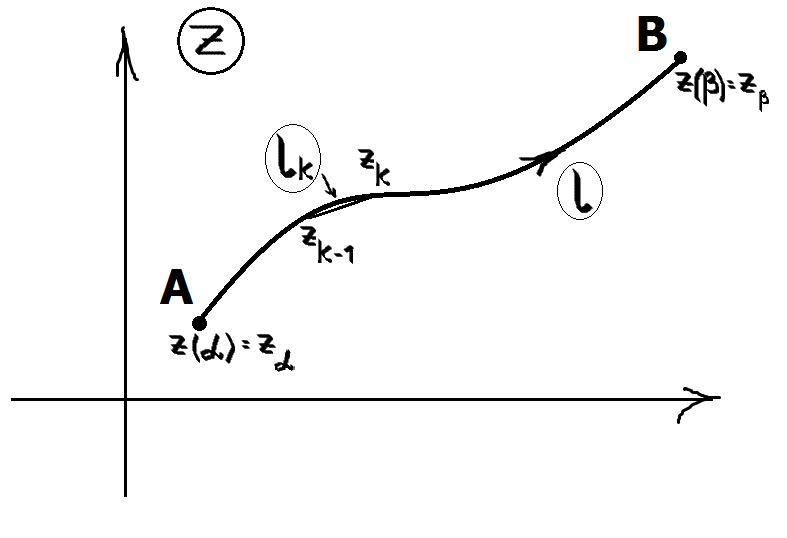
\includegraphics[height=0.4\textwidth]{lec30_9.png}}

Пусть $d = max |\Delta z_k|,\ \text{где } \Delta z_k = z_k - z_{k-1}, 
k = \overline{1, n}.\ d - \text{диаметр, }d = \diam\ P$ нашего разбиения $P$ 
точками $z_i, i = \overline{0, n}.$ На каждой дуге разбиения $l_k$ 
выберем отмеченные точки $M_k \in l_k, k = \overline{1, n}.$ 
Если на исходной кривой определена функция $w = f\left(z\right), $ то в 
соответствии с использованным разбиением $P$ с множеством отмеченных точек
$S = \{M_k\}_{k=1}^n$ можно составить 
\begin{equation}
    \label{lec30_2:2}
    \sigma = \sigma\left(f, \{P, S\}\right) =
    \sum_{k=1}^{n}{f\left(M_k\right)\Delta z_k}
\end{equation}
Функция $f\left(z\right), z \in l, $ называется интегралом на $l$, если
$\exists\ I \in C:$

\begin{equation}
    \label{lec30_2:3}
    \forall \eps > 0 \quad \exists \delta = 
    \delta_\eps > 0 : 
    \forall \{P, Q\},\ d = \diam\ P \leq \delta \implies
    |\sigma - I| \leq \eps.
\end{equation}

Здесь число $I \in C$ будем называть значением интеграла ФКП
$f\left(z\right)$ по $l$ и обозначать 
\begin{equation}
    \label{lec30_2:4}
    I = \int\limits_l{f\left(z\right) dz} \stackrel{\eqref{lec30_2:2}}{=}
    \lim_{d \to 0}\sigma = \lim_{d \to 0}{\sum_{k=1}^n{
    f\left(M_k\right)\Delta z_k}}
\end{equation}
Определение интеграла ФКП соответствует определению КрИ-2 для
действительных функций.

Пусть $f\left(z\right) = c_0 = const \in C$
$\sigma \stackrel{\eqref{lec30_2:2}}{=} \sum\limits_{k=1}^n{c_0\Delta z_k} = 
c_0\left(-z_0 + z_1 - z_1 + z_2 - \ldots - z_{n-1} + z_n\right) = 
c_0\left(z_n - z_0\right) = c_0\left(z_\beta - z_\alpha\right)$

В частности, если $c_0 = 1,$ то
$\int\limits_{\overbow{z\left(\alpha\right)z\left(\beta\right)}}{dz} = 
z\left(\beta\right) - z\left(\alpha\right)$

Если же $c_0 = 0, $ то
$\int\limits_{\overbow{z_\alpha z_\beta}}{0dz} = 0$

Для вычисления интеграла ФКП через КрИ-2 от действительной функций 
рассмотрим функции Ф2П

\begin{equation*}
 \begin{cases}
  u = u\left(x, y\right) = \Re f\left(z\right)\\
  \quad v = v\left(x, y\right) = \Im f\left(z\right)
 \end{cases}
\end{equation*}

В соответствии   с используемым разбиением точками $P = \{z_k\}$ с
отмеченными точками 
$S = \{M_k = M_k\left(x(\tau_k), y(\tau_k)\right)\}, $ а 
$\{t_k\}_{k=1}^n $~--- соответствующие точки разбиения 
$\left[\alpha,\beta\right],$ то рассматриваемую интегральную сумму 
$\eqref{lec30_2:2}$ запишем в виде

$\sigma = \sum\limits_{k=1}^n{\left(u(x(\tau_k), y(\tau_k))
+ iv(x(\tau_k), y(\tau_k))\right)\left(\Delta x_k + 
i\Delta y_k\right)}, \text{где }$ \\
$\Delta x_k = x\left(t_k\right) - 
x\left(t_{k-1}\right),$ \\ $\Delta y_k = y\left(t_k\right) - 
y\left(t_{k-1}\right)$

Отделяя действительную и мнимую части, имеем
\[
\sigma =    \sum_{k=1}^n{\left(u(x(\tau_k), y(\tau_k)\right)\Delta x_k -
v\left(x(\tau_k), y(\tau_k)\right)\Delta y_k} + 
i\sum_{k=1}^n{u\left(x(\tau_k), y(\tau_k)\right)\Delta y_k + 
v\left(x(\tau_k), y(\tau_k)\right)\Delta x_k}
\]
Переходя к пределу 
$d = \underset{1 \leq k \leq n}{max}|\Delta z_k| = 
\underset{1 \leq k \leq n}{max}\sqrt{\Delta x_k^2 + \Delta y_k^2}
\longrightarrow 0 \implies
\begin{cases}
    \Delta x_k \longrightarrow 0\\
    \Delta y_k \longrightarrow 0
\end{cases}$

получаем в силу определения КрИ-2 для действительных Ф2П
\[
\sigma \underset{d \to 0}{\longrightarrow} \int\limits_l{
udx - vdy} + i\int\limits_l{udy + vdx}, \text{т.~е.}
\]
\begin{equation}
    \label{lec30_2:5}    
    \int\limits_{l}{f\left(z\right)dz} = \int\limits_l{udx - vdy} + 
    i\int\limits_l{udy + vdx}
\end{equation}
\eqref{lec30_2:5} можно также формально получить следующим образом 
\[
f\left(z\right) = u + iv, \quad
dz = dx + idy
\int\limits_l{\left(u+iv\right)\left(dx + idy\right)} = 
\int\limits_l{udx - vdy} + i\int\limits_l{udy + vdx} 
\iff \eqref{lec30_2:5}.
\]

В частности, если $l$ имеет параметризацию $\eqref{lec30_2:1},$ то в 
этом случае 

$I = \left[
\begin{array}{ccc}
     x = x\left(t\right)\quad dx = x^\prime\left(t\right)dt \\
     y = y\left(t\right)a\quad dy = y^\prime\left(t\right)dt \\
     \alpha \leq t \leq \beta\\
\end{array} 
\right]=
$

$
\stackrel{\eqref{lec30_2:5}}{=}
\int\limits_\alpha^\beta{\left(u(x(t), y(t))x^\prime(t) - 
v(x(t), y(t))y^\prime(t)\right)dt} + i\int\limits_\alpha^\beta{
\left(u(x(t), y(t))y^\prime(t) + v(x(t), y(t))x^\prime(t)\right)dt}
$

\begin{example}
    Пусть $n \in Z.$ Рассмотрим 
    $I_n = \int\limits_{|z-z_0| = R}{\frac{dz}{\left(z-z_0\right)^n}}$\\
    Используем параметр этой окрестности $z=z_0 + R e^{it}, \
    0 \leq t \leq 2\pi,$ имеем
    $dz = iRe^{it}dt$\\
    Значит, $I_n = \int\limits_0^{2\pi}{\frac{iRe^{it}dt}{
    (R e^{it})^n}} = \frac{i}{R^{n-1}}\int\limits_0^{2\pi}{
    e^{(1-n)it}dt}$\\
    Если $n \neq 1, $ то $I_n = \frac{i}{R^{n-1}}\frac{
    e^{(1-n)it}}{(1-n)i}\bigg|_0^{2\pi} = \frac{
    (e^{2\pi i(1-n)}-1)}{R^{n-1}(1-n)} = 0$
    
    Для $n=1 \implies I_1 = i\int\limits_0^{2\pi}{dt} = 2\pi i$\\
    Таким образом получаем 
    \begin{equation}
        \label{lec30_2:6}
        \int\limits_{|z-z_0| = R}{\frac{dz}{(z-z_0)^n}} = 
        \begin{cases}
            0,\ n \neq 1 \in Z\\
            2i\pi,\ n = 1
        \end{cases}
    \end{equation}
\end{example}

Из полученной формулы вычисления интеграла ФКП через соответствующие
действительные КрИ-2 на основании основных свойств КрИ-2 получим 
следующие свойства интеграла ФКП:

\begin{enumerate} 
  \item  Зависимость от выбранной ориентации пути: 
$\int\limits_{\overbowright{AB}}{f\left(z\right)dz} = 
-\int\limits_{\overbowright{BA}}{
f\left(z\right)dz}$

\item Линейность. Если $f, g $~--- интегрируемы на $l$ в 
комплексной плоскости, то тогда \\
$\forall\ \lambda, \mu \in C \implies \exists \int\limits_l{\left(
\lambda f + \mu g\right)dz} = \lambda\int\limits_l{fdz} + 
\mu\int\limits_l{gdz}$

\item Аддитивность.
Если $l = l_1 \cup l_2,$ причём $l_1$ и $l_2$, во-первых, имеют общие
только граничные точки и, во-вторых, ориентированы так же, как $l$, то
тогда для интегрируемой на $l$ ФКП имеем: \\
$\int\limits_{l_1\cup l_2}{f\left(z\right)dz} = 
\int\limits_{l_1}{f(z)dz} + \int\limits_{l_2}{f(z)dz}$

\item  Основная оценка интеграла ФКП.
Если $f\left(z\right)$ интегрируема на $l$, то \\
$|\int\limits_l{f\left(z\right)dz}| \leq \int\limits_l{
|f\left(z\right)||dz|} $~--- КрИ-1, где
$|dz| = \sqrt{dx^2 + dy^2} $~---  дифф. дуги.

Доказательство следует из соответствующей оценки для 
$\eqref{lec30_2:2}$:\\
$|\sigma| \stackrel{\eqref{lec30_2:2}}{=} 
|\sum\limits_{k=1}^n{f\left(z(t_k)\right)\Delta z_k}| \leq 
\sum\limits_{k=1}^n{|f\left(z(t_k)\right)||\Delta z_k|}
\underset{d \to 0}{\to} \int\limits_l{|f\left(z\right)||dz|}$\\
В частности, из основной оценки, полагая $M = 
\underset{z\in l}{\sup}|f\left(z\right)|$\\
$|\int\limits_l{f\left(z\right)dz}| \leq \int\limits_l{M|dz|} = 
M\int\limits_l{|dz|} = M\ \text{Длина}\ l = Ml_0$, где $l_0 $~--- длина $l.$
\end{enumerate}

\section{Интеграл ФКП от аналитической ФКП}
Напомним, что $f\left(z\right)$ считается аналитической в $D \in C, $
если она дифференцируема в каждой точке $D$($D$~--- область).\\
Так как далее будет понятно, что из существования производной первого
порядка ФКП следует существование всех производных высших порядков этой
ФКП, то аналитическая функция будет бесконечное число раз непрерывно 
дифференцируема на $D.$

\begin{thm}[Интегральная теорема Коши]
Если $f\left(z\right)$ непрерывно дифференцируема в односвязной области
$D \in C,$ то тогда для любого замкнутого кусочно-непрерывного контура
\end{thm}
\begin{equation}
    \label{lec30_2:7}
    \oint\limits_l{f\left(z\right)dz} = 0.
\end{equation}
\end{document}  
